\documentclass[12pt,a4paper]{article}
\usepackage{amsmath, amssymb, geometry}
\geometry{margin=1in}
\usepackage{siunitx}
\usepackage{bm}
\usepackage{hyperref}
\usepackage{url}
\usepackage{graphicx}
\usepackage{subcaption}

\title{Week 07 Assignment Based on Book Computer Vision by Richard Szeliski, Second Edition, Chapter 9}
\author{Bishwash Khanal, \texttt{bishwash.b.khanal@student.jyu.fi}}
\date{October 26, 2025}

\begin{document}

\maketitle

\section{Transparent motion and reflection estimation}
Take a video sequence from your phone (maximum 30 second clip) looking through a window (or picture frame) and see if you can remove the 
reflection to better see what is inside. The steps are described in Section 9.4.2.

Also, submit your original video clip taken and source code to remove reflection which can be run.

Optional: Try above with video clips taken through transparent window during the day, and during the night. You may also take the clip 
through car window during this day and the night. Report the differences in results and the impact of lightening effect.
\newline
\textbf{Original Video Clip:} \href{https://drive.google.com/file/d/1gjEgFKrlBo2PgFSqi23-u5K3uIAr0AF5/view?usp=sharing}{Google Drive}
\newline
\textbf{Notebook:} \href{https://colab.research.google.com/drive/1H8oc060oYT3zyzLS-TISJCzxbsjmcvuA?usp=sharing}{Assignment\_Week7\_Q1.ipynb (Google Colab)} - 
\href{https://github.com/bkhanal-11/ties411_cvip_jyu/blob/master/assignment7/src/Assignment_Week7_Q1.ipynb}{(GitHub)}

\begin{figure}[htb]
    \centering
    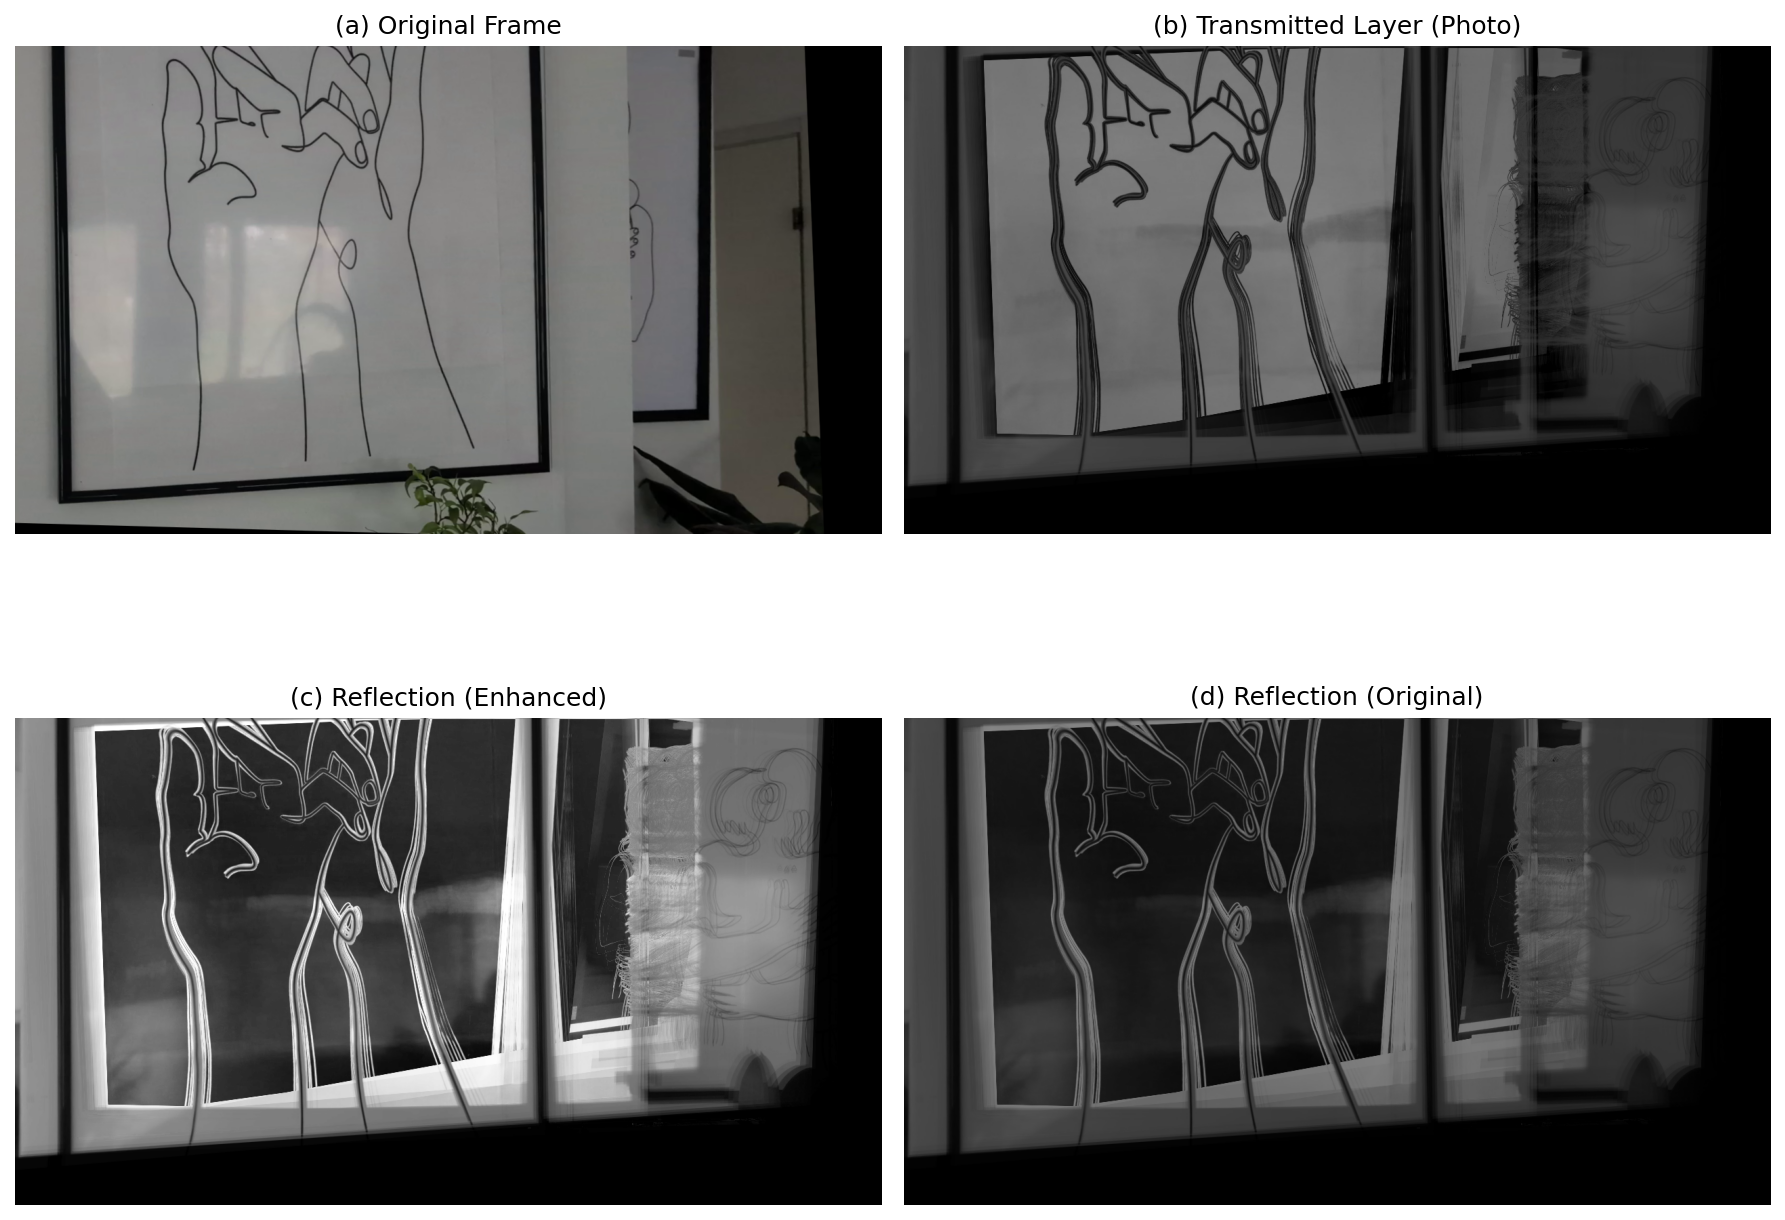
\includegraphics[width=0.95\textwidth]{src/reflection_removal_results.png}
    \caption{Results of Reflection Removal from Video Frames}
    \label{fig:comparison}
\end{figure}



\section{Optical Flow}
Write a simple program to track silver colored Honda Civic hatchback car (the very first car you see) in the given video clip. 
Link to video clip: \url{https://drive.google.com/file/d/1p2g68kxvXnez9yc2nhD6XJ0aGTx2tyRX/view?usp=sharing}

Implement one sparse optical flow based method and one dense optical flow based method.

Deliverable: 1) source code which takes the given video as input and implements both methods, 2) Output: tracked outcome from both methods, 
3) Your analysis on the result. Merits and demerits of each method over another.

Hint (recommended to check this before attempting this question): \url{https://docs.opencv.org/3.4/d4/dee/tutorial_optical_flow.html}


\subsection{Results}

\textbf{Notebook:} \href{https://colab.research.google.com/drive/1e2mMba6YOY2pt4cyBrOAsf8wfL6rVag4?usp=sharing}{Assignment\_Week7\_Q2.ipynb (Google Colab)} - 
\href{https://github.com/bkhanal-11/ties411_cvip_jyu/blob/master/assignment7/src/Assignment_Week7_Q2.ipynb}{(GitHub)}
\newline
Sparse Optical Flow Output: \href{https://drive.google.com/file/d/1iLkjQO8ZW9hpywKb2z5pnCL-cukpZUon/view?usp=sharing}{Google Drive}
\newline
Dense Optical Flow Output: \href{https://drive.google.com/file/d/1LyLgQWyLzUiwqHsQQL1IQbtPpALp8bBU/view?usp=sharing}{Google Drive}

\begin{figure}[htb]
    \centering
    \begin{subfigure}[b]{0.48\textwidth}
        \centering
        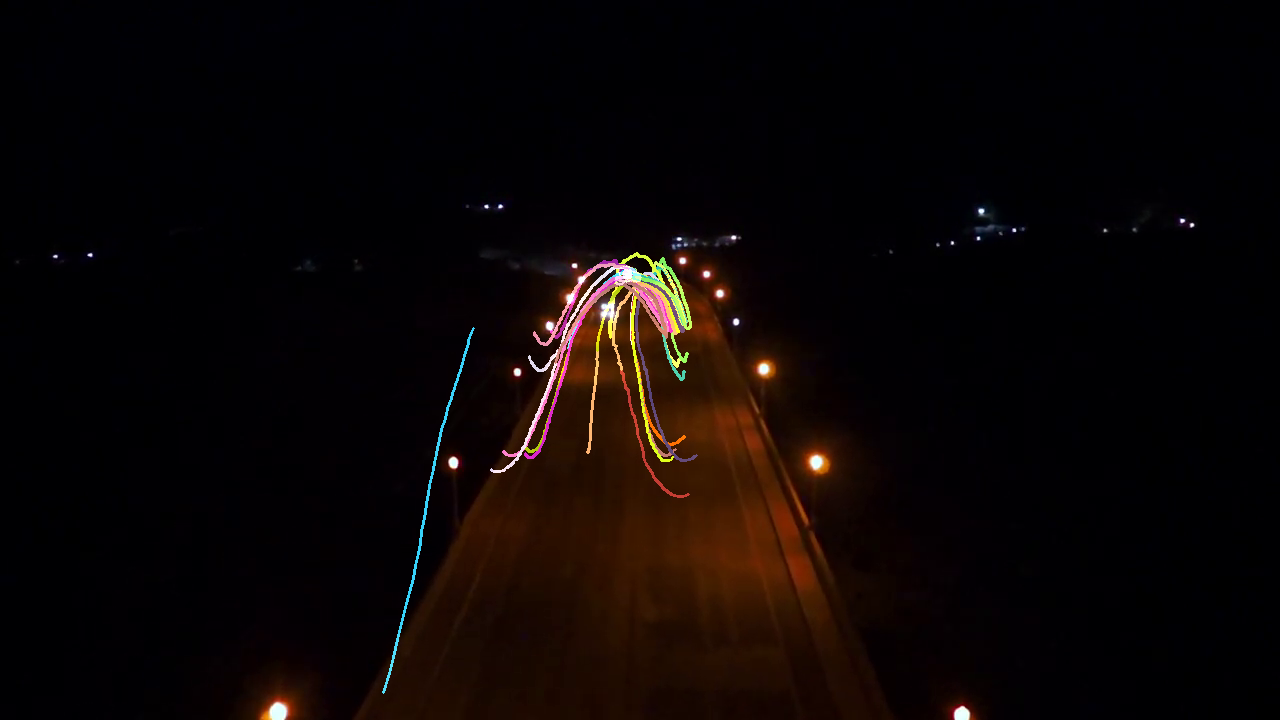
\includegraphics[width=\textwidth]{src/sparse_last_frame.png}
        \caption{Sparse Optical Flow Tracking}
    \end{subfigure}
    \hfill
    \begin{subfigure}[b]{0.48\textwidth}
        \centering
        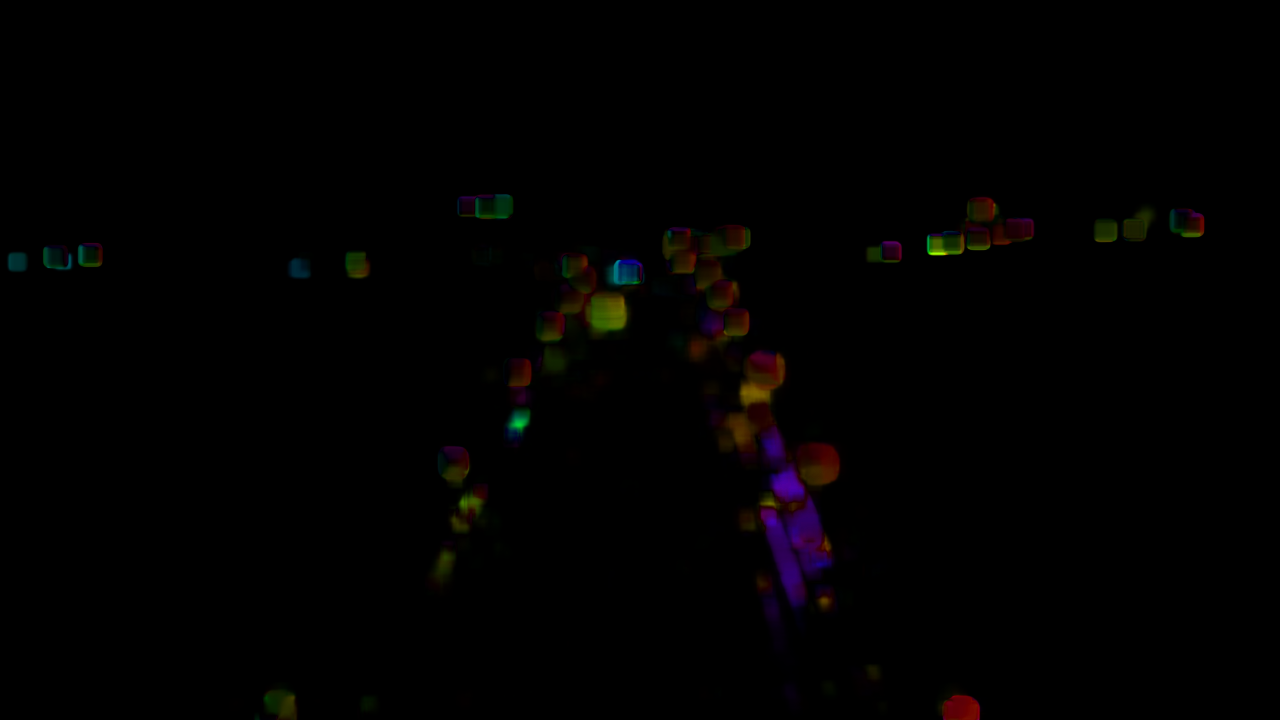
\includegraphics[width=\textwidth]{src/dense_last_frame.png}
        \caption{Dense Optical Flow Tracking}
    \end{subfigure}
    \caption{Comparison of Optical Flow Tracking Methods \textit{(Last Frame)}}
\end{figure}

\subsection{Analysis}
\textbf{Sparse Optical Flow} method initially tracked the car well, especially when it was close to the camera as its corner features (like headlights and edges) were 
clearly visible. The motion trajectories were clean and stable in the earlier frames. This demonstrates the method's efficiency under good conditions. 
However, as the car moved farther away and became smaller and blurrier, some of feature points began to disappear. Tracking looks to have degraded, 
with some of the points getting lost. Sparse flow proved fast and responsive but struggled with the reduced visibility and gradual occlusion caused 
by low light and distance.

In contrast, \textbf{Dense Optical Flow} approach maintained a more consistent tracking throughout the video. It captured the car's movement 
even as it became less defined, leveraging pixel-wise motion estimation across the entire frame. This allowed it to better follow the vehicle 
during its fade-out phase, despite the low texture and lack of sharp features. However, this came at a cost—processing was slower, 
and some noise was introduced due to background motion and low lighting conditions. Unlike Sparse Optical Flow, we cannot select a region of interest and 
the whole frame is tracked hence this is not optimal for a moving camera.

\end{document}
